The service supports website admins to host and administer Drupal websites directed to the grand public,
such as experiment or departmental central websites.
Some of the most popular sites based on this service are \href{https://home.cern/}{home.cern}, \href{https://atlas.cern}{atlas.cern},
\href{https://cms.cern}{cms.cern}, \href{https://careers.cern}{careers.cern} and \href{https://visit.cern}{visit.cern}.
They form CERN's main outreach channel and are critical for the Organization's reputation.

Users of the service range across a wide spectrum of different professional profiles,
and it's quite common that the responsibility of site building at CERN falls on administrative personnel, or personnel with little technical background in web technologies.
This in turn shapes the kind of service we have to provide; it is, for example, impractical to rely on developer-centric workflows, like GitOps and CLI tools.
A small fraction of our user base, however, indeed have web development experience.

The consequence is that the Content Management service has a dual mission:
\begin{enumerate}
    \item to ensure the \emph{high availability} and performance of these communication channels
    \item to make site building and administration accessible to a wide-ranging user base, while remaining extensible for websites needing special features
\end{enumerate}

%This work describes an infrastructure project that focuses on furthering the \emph{first mission}, without sacrificing the second.
%Ideally, the changes should be almost transparent for non-technical site administrators, while enabling previously unavailable best-practices workflows for technical users.

\subsubsection*{Control vs. customization}

%All websites on the infrastructure are running the same Drupal distribution in a "multi-site" configuration, as will be explained in section \ref{sec-phys-infra}.
%The distribution consists of an upstream Drupal version with a few patches for the CERN environment, plus a curated set of "central" modules.
Curating the Drupal distribution, and critically, the application of \emph{security updates}, is the responsibility of the infrastructure team.
However, many websites need extra features and Drupal was selected exactly \hyperref[drupal-at-cern]{because of its extensibility}.
Website admins should be able to use community modules, thereby extending Drupal specifically for their website -- and assuming limited responsibility to keep custom code secure.

\subsection{Load characteristics}
\label{sec-load}

\href{https://home.cern/}{home.cern} is the most popular website at CERN, as shown in figure \ref{fig-drp-top10-cip}.
Out of \emph{1043} Drupal websites currently hosted, it alone serves 32\% of monthly unique visitors.
The top 10 websites together serve 79\% of all unique visitors, leaving only 1/5 of them headed for the other 1033 websites.
This is an intrinsic characteristic of the service load, which is heavily skewed towards a very small number of critical websites.

\begin{figure}[t]
    \centering
    \vspace{-3em}
    \begin{subfigure}[b]{.7\textwidth}
        \centering
        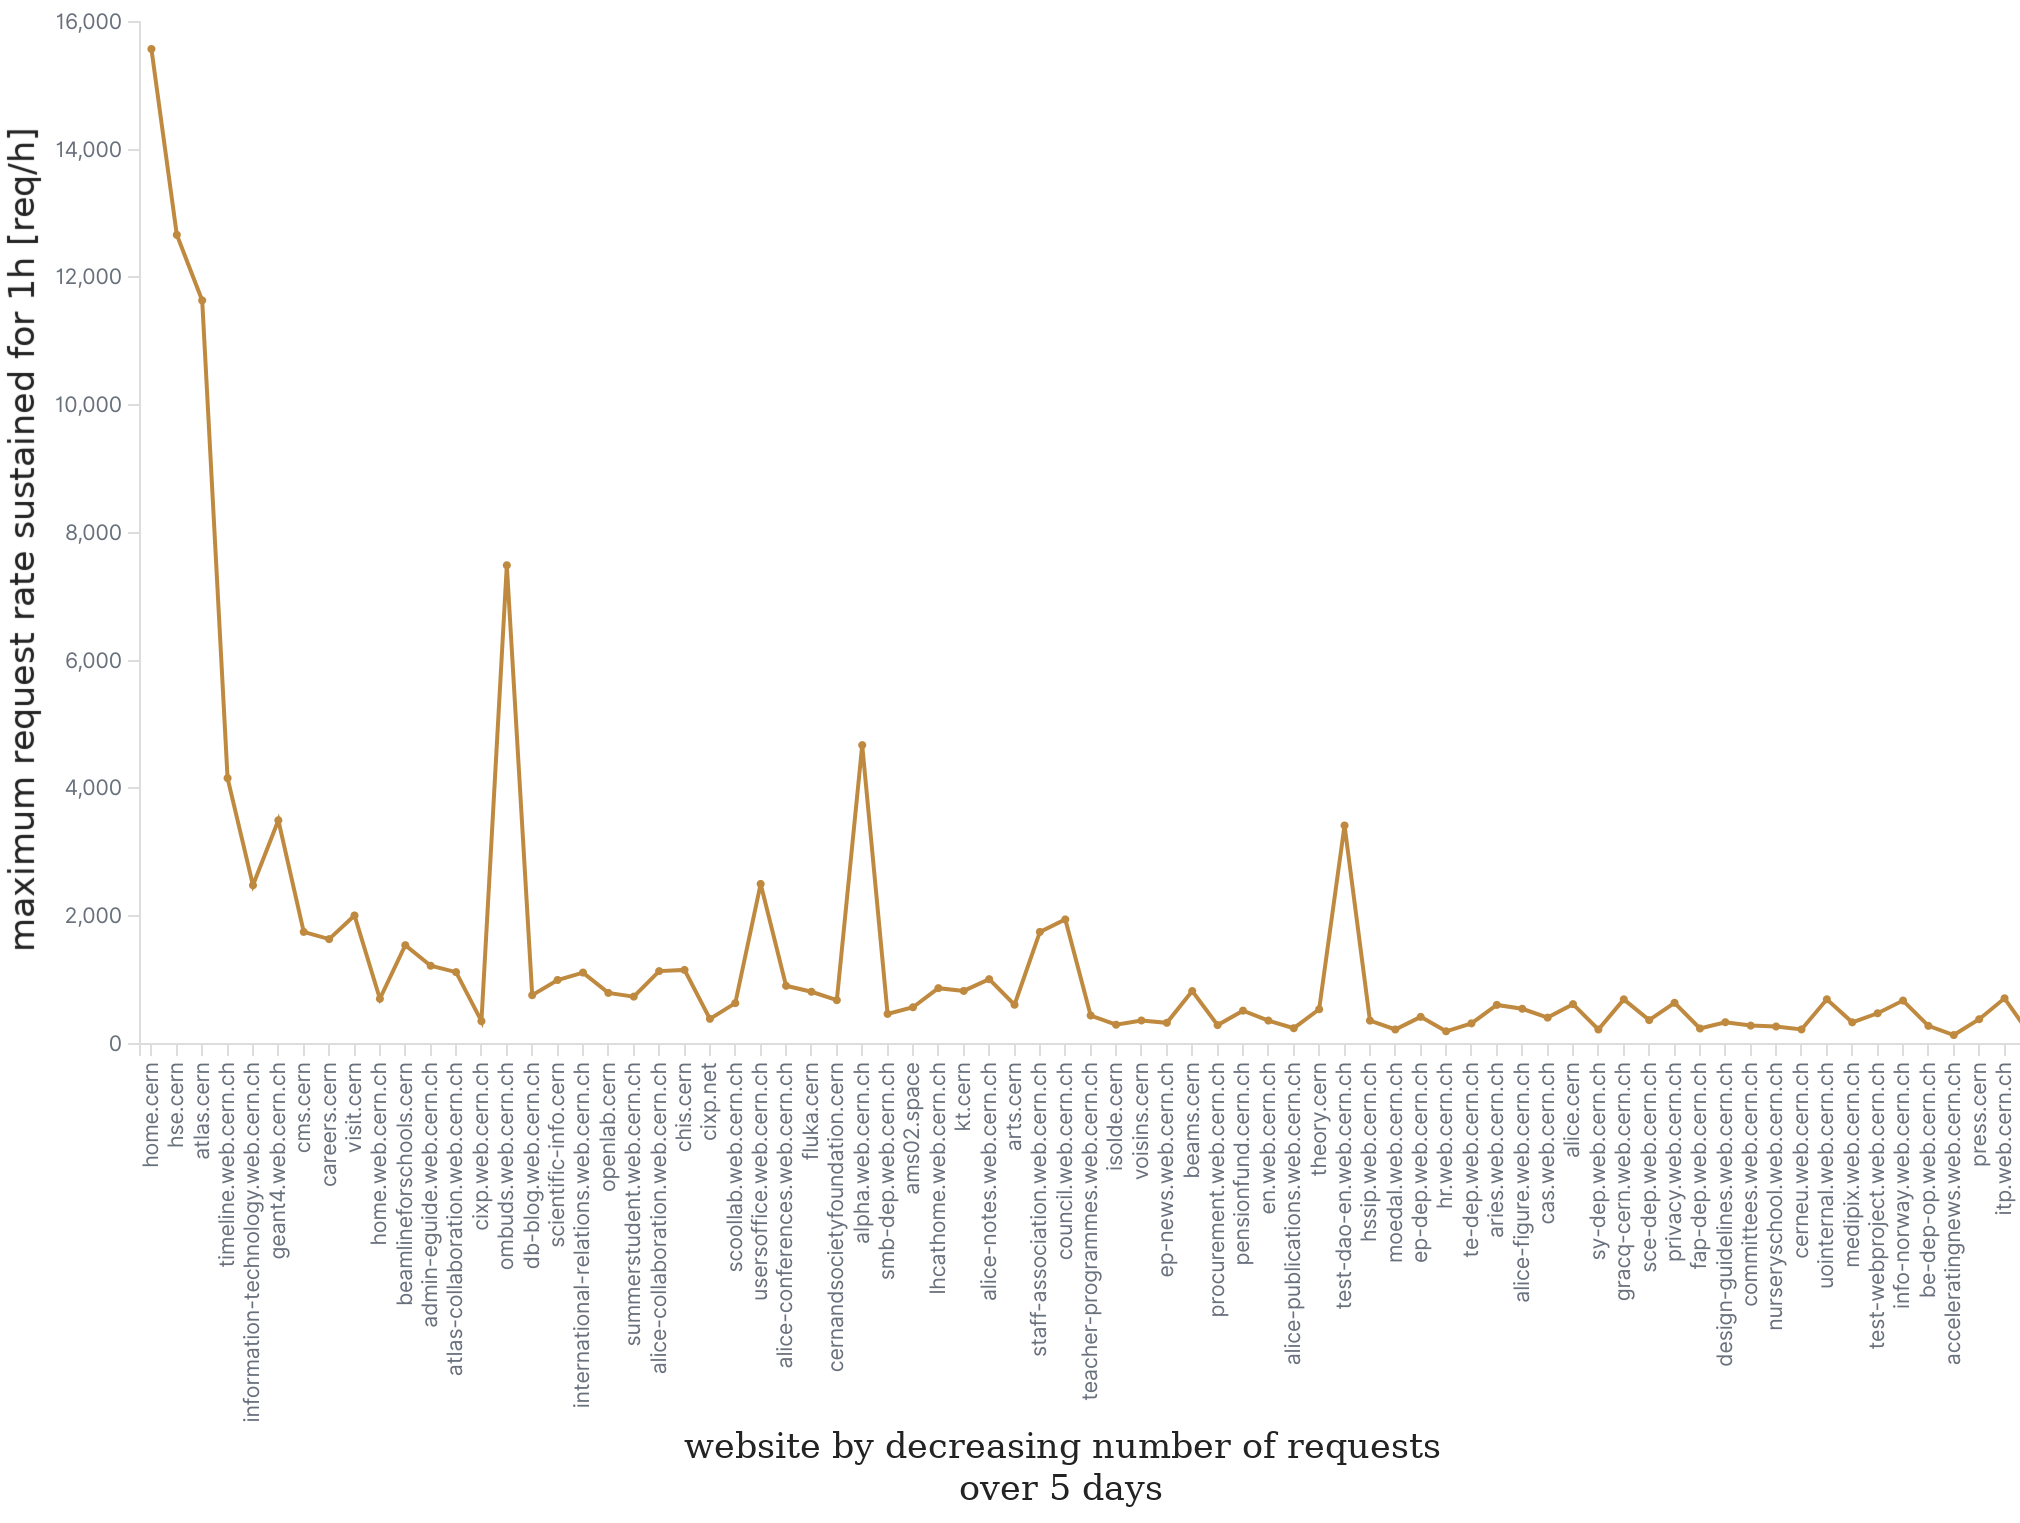
\includegraphics[width=\textwidth]{figures/website-bandwidth}
        \caption{\emph{Maximum sustained throughput for high traffic websites}.
          The maximum throughput of the highest traffic websites was recorded over a period of 5 days.
          The websites with the highest traffic also have the highest throughput, showing that sustained bursts of traffic are uncommon.}
        \label{fig:website_bandwidth}
    \end{subfigure}
    \hfill
    \begin{subfigure}[b]{.25\textwidth}
    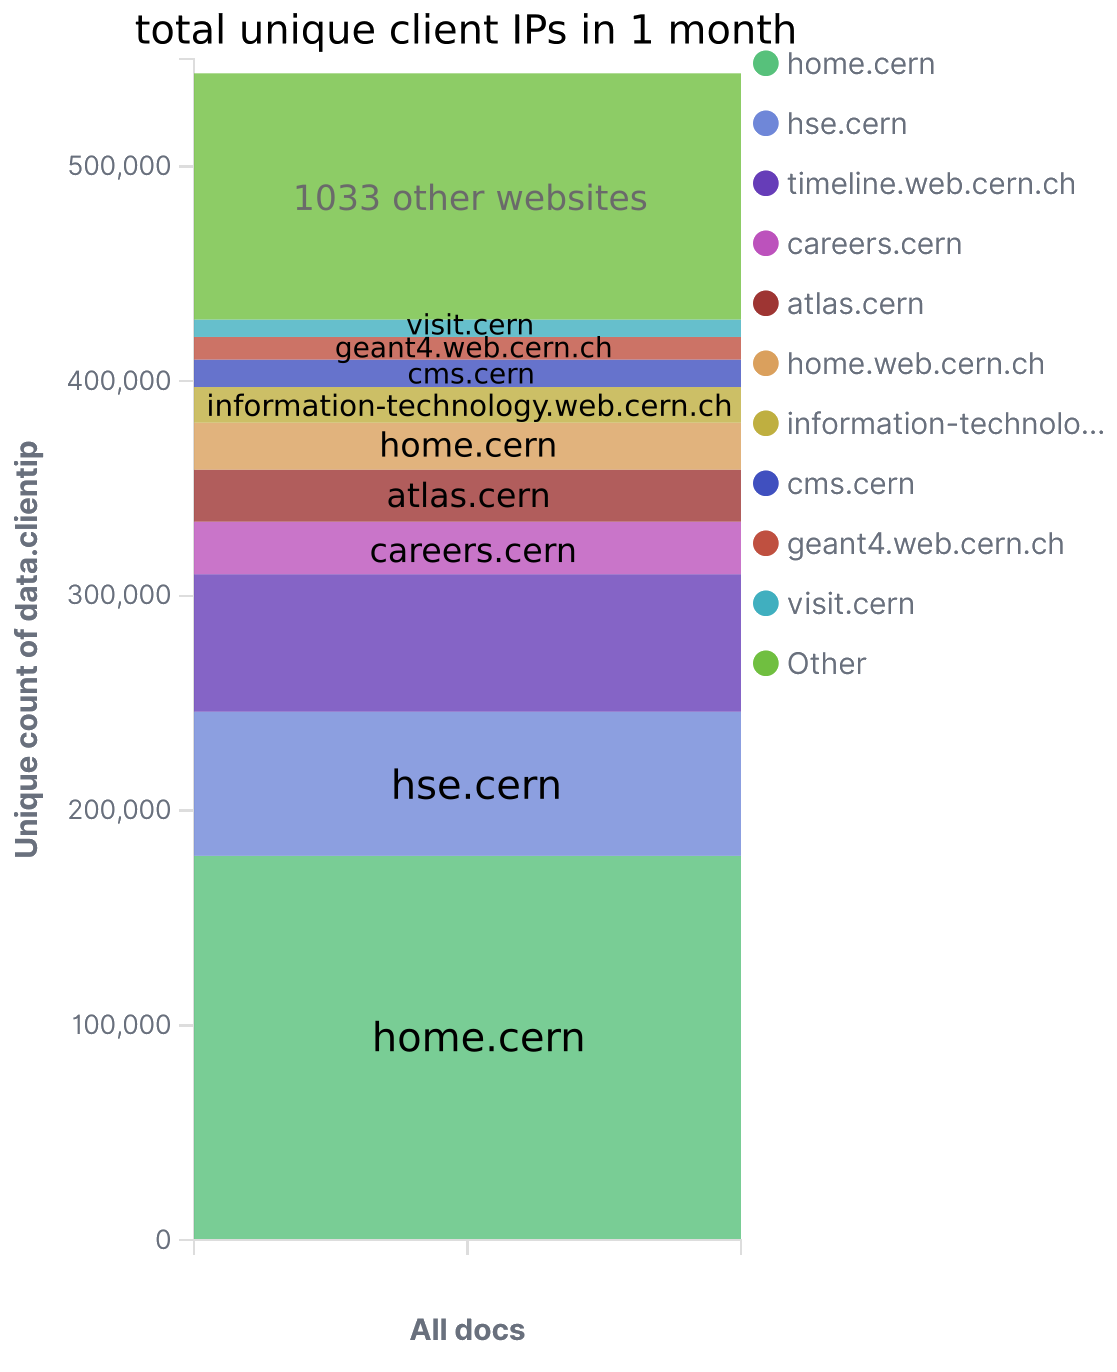
\includegraphics[width=\textwidth]{figures/drupal-top10-uniqClientIP.png}
    \caption{\emph{Public outreach}: 
        The top 10 most popular Drupal websites are shown.
        home.cern appears twice as \texttt{home.cern} and \texttt{home.web.cern.ch}.
        {\color{amethyst} \texttt{timeline.web.cern.ch}} has machine traffic.}
    \label{fig-drp-top10-cip}
    \end{subfigure}
    \vspace{-1.8em}
    \caption{Load characteristics}
    \vspace{-2em}
\end{figure}

Unique visitors over 1 month are taken as a measure of a site's popularity, or how much impact it has on the Organization's reputation,
but a measure more suitable to assess an infrastructure on is the rate of HTTP requests.
In section \ref{sec-experiment} we will describe an experiment on resource optimization in the Kubernetes infrastructure
by assigning websites to different Quality of Service classes.

The 10 websites with the highest traffic are the target of 60\% of all requests, and they have a high overlap with the most popular sites (fig. \ref{fig:website_bandwidth}).
The most popular websites therefore, apart from the highest availability guarantees, need also the highest throughput.

What sustained rate of requests should a website be able to handle with stable response time?
To better understand how the load impacts a single website (and therefore estimate the required hosting resources),
we performed the measurements of figure \ref{fig:website_bandwidth}.

These observations align with expectations and requirements: critical websites should be able to handle a throughput of 40 requests per second with stable response times.